%!xelatex
\documentclass[main.tex]{subfiles}
\begin{document}

\chapter{Introduction}\label{chp:introduction}

\section{Product Overview}

\term*{Crochet} is a method to turn yarn into textiles. It is a form of art that uses a crochet hook to knot the yarn in such a way to produce a three-dimensional product, which can range from clothing and toys to bags and public art displays.
A crochet \term*{pattern} is a list of steps to produce a specific product, analogous to a cooking recipe. The design of crochet patterns typically involve many iterations of producing, refining, and experimenting, and the \CC{} app attempts to simplify this process.

\CC* is a web application that produces real-time 3D visualizations of crochet patterns. It allows designers to input their textual pattern and view the simulated product resulting from the pattern. Designers can refine and iterate on their pattern without the time-consuming process of constructing the design in the real world each time.

\section{First Sample Run}

Start the \CC{} application by opening \href{https://crochetcraft.jtai.ca}{\io{crochetcraft.jtai.ca}} in your web browser. Once loaded, the application's \ScLayout{} is shown in figure~\ref{fig:layout}. Left mouse click anywhere in the pattern text box, and type or copy-and-paste the following pattern:

\io{%
    0. ch 11 \\
    1. sc 10 \\
    2-10. ch 1, turn, sc 10 \\
    ch 1
}

After all of the above text has been inserted, a 3D visualization of the pattern will be displayed in the rendering area. Next, use the mouse to highlight the text \io{2-10} in the pattern text box, and overwrite it by typing \io{2-20}. The modified pattern will be visualized in the rendering area.

\begin{figure}[htbp]
    \centering
    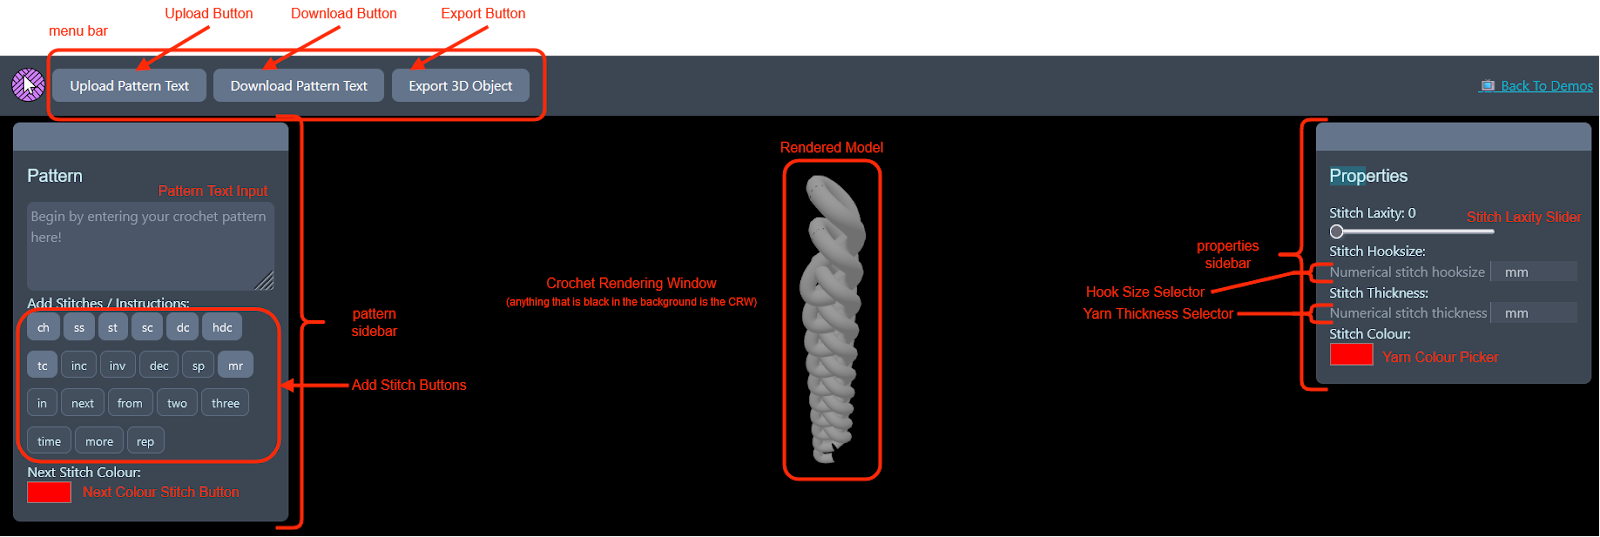
\includegraphics[width=\linewidth]{layout.png}
    \caption{\ScLayout{} of \CC.}
    \label{fig:layout}
\end{figure}

\end{document}
